\chapter{Implementierung}\label{chap:impl}

Dieses Kapitel beinhaltet den Hauptteil der Arbeit. Es geht um die konkrete Implementierung des Emulators und alle bisher genannten Bestandteile. Die folgenden Inhalte sind entsprechend den Modulen im Quellcode gegliedert und bieten einen breiten Überblick über unterschiedliche Umsetzungen.

\section{Emulator}

Die Entwicklung des Emulators basierte größtenteils auf einer ordentliche Wiedergabe der Spezifikation des 8080s, an dessen Vorgaben sich gehalten werden musste. Dementsprechend sind im folgenden die Implementierung der Register und der \ac{API} für die Ein- und Ausgabegeräte dargestellt.

\subsection{Registerarray}

Im folgenden werden drei Aspekte der Implementierungen des Registerarrays gezeigt: Die Repräsentation und der Zugriff auf die Register, sowie der Zugriff auf die Flags.

\subsubsection{Datentyp}

Naive Implementierungen eines Registerarrays würden die Register einzeln implementieren und für Registerpaare die entsprechenden Inhalte konkatenieren.
Dies ist jedoch unnötig umständlich. Der effizientere Ansatz ist die Register in Paaren zu speichern (als 16-Bit Unsigned Integer) und die Möglichkeit beizubehalten, die beiden Bytes individuell anzusprechen. In einer Sprache wie C ist dies mit Pointer-Arithmetik gut lösbar, in Rust ist es sinnvoller ein Union zu verwenden.

\begin{minted}{rust}
#[repr(C)]
union Register {
    bytes: (u8, u8),
    value: u16,
}
\end{minted}

Ein Union wird ähnlich wie ein Struct deklariert, jedoch teilen alle Felder den gleichen Speicherplatz\footnote{ausführliche Erklärung: \url{https://doc.rust-lang.org/reference/items/unions.html}}. Das bedeutet man kann den Wert eines solchen \rust{Register} entweder durch \rust{Register::bytes} als Tupel aus 2 Bytes oder durch \rust{Register::value} als 16-Bit-Wert auslesen. Dadurch ist keinerlei Konkatenation der Registerwerte notwendig.

\subsubsection{Registerzugriff}

Der Registerzugriff ist eine sehr häufig verwendete Operation, da ein großer Teil der zu implementierenden Instruktionen sie benötigt. Um dies möglichst einfach zu machen, wurde Indizierung für den Registerarray implementiert. Über String-Indizierung --- \rust{reg["bc"] // Registerpaar BC} --- ist der Zugriff auf Registerpaare geregelt, über Character-Indizierung --- \rust{reg['b'] // Register B} --- der normale Zugriff.

\subsubsection{Zugriff auf Flags}

Die Flags sind bekannterweise Teil des \ac{PSW}-Registerpaars, sprich sie sind als ein einzelnes Byte gespeichert. Um die Werte der einzelnen Flags zu erhalten, werden Bitmasken verwendet. Um bspw. herauszufinden, ob das Bit mit dem höchsten Stellenwert gesetzt ist, muss der Ausdruck \rust{byte & 0x80 != 0} berechnet werden. Wenn dieser \rust{true} ist, ist das Bit gesetzt\footnote{\rust{0x80 == 0b10000000}}.

\subsection{Ein-/Ausgabegeräte}

Wie im \cref{chap:design} zu sehen ist, beinhaltet die zentrale Struktur zwei Arrays aus 256 Elementen, um Ein- und Ausgabegeräte zu realisieren. Der Übersichtlichkeit halber wurde der Datentyp dieser Arrays vereinfacht. Bei der Umsetzung als Array ist es problematisch, dass initial keine Geräte registriert sind, der Array also leer wäre. Da es in Rust kein \rust{null} gibt, muss der Array mit dem \rust{Option}-Typ befüllt werden:

\qquad\rust{[Option<InputDevice>; 256]}

Diese Implementierung ist jedoch noch immer ungenügend, weil verschiedene Geräte registriert werden können. In klassischen objektorientierten Sprachen wären deshalb Input- bzw. OutputDevice als Interfaces realisiert, analog dazu gibt es in Rust Traits (siehe \cref{chap:prereqs}). Da die Größe von Trait-Objekten nicht zur Compilezeit bestimmt werden kann, kann ein solches Objekt nicht auf dem Stack gelagert werden, was für die Initialisierung der eigentlichen Arrays aber  erforderlich ist. Deshalb muss ein Pointer verwendet werden. Rust verwendet sogenannte \glqq Smartpointer\grqq{} um die klassischen Probleme bei Verwendung von Pointern zu vermeiden. Meistens wird der Typ \rust{Box} genutzt, der es allerdings verhindert Daten mehrfach zu referenzieren. Diese Möglichkeit ist jedoch notwendig, da sowohl von außen, als auch von innen mit den Geräten kommuniziert werden muss. Durch Kombination von \rust{Rc}, einem referenzzählendem Pointer, mit \rust{RefCell}, einer schreibbaren Speicherregion, kann das gewünschte Verhalten erreicht werden. Die Syntax um einen derartigen Array zu deklarieren ist wie folgt:

\qquad\rust{[Option<Rc<RefCell<dyn InputDevice>>>; 256]}

Solange das Programm als einzelner Thread ausgeführt wird, kann nun jederzeit mit einer mutable (\textit{veränderbaren}) Referenz auf ein solches InputDevice gearbeitet werden. Außerdem dürfen beliebig viele non-mutable Referenzen existieren, sofern im aktuellen Scope keine mutable Referenz auf das Gerät existiert.

\section{Assembler}

Die Implementierung des Assemblers besteht aus drei maßgeblichen Komponenten: Dem eigentlichen Assembler, dem im Code sogenannten \enquote{preprocessor} zur Vorverarbeitung und einem Parser für numerische Eingaben des Nutzers. In den folgenden Abschnitten wird auf verschiedene Besonderheiten und Herausforderungen der drei Komponenten eingegangen, was mittels Code-Beispielen illustriert wird. Generell gilt, dass der führende und schließende Whitespace einer Zeile des Programmcodes vor deren Behandlung durch die Methode \rust{.trim()} entfernt und die Zeile gegebenenfalls übergangen wird, sofern eine Leerzeile entsteht. Der Übersichtlichkeit halber ist dieser Teil des Codes an vielen Stellen ausgelassen.

\subsection{Assembler.rs}

Der in der Klasse \rust{assembler.rs} definierte Struct 
\begin{minted}{rust}
    pub struct Assembler {
        code: Vec<String>,
    }
\end{minted}
bildet die Schnittstelle für den eigentlichen Emulator und das \ac{WASM}-Interface. Der Emulator benötigt den zu Bytecode übersetzten Input des Nutzers und liefert dem Assembler dafür bei der Initialisierung ein String-Slice, das diesen Input repräsentiert. Basierend darauf erzeugt der Assembler das Objekt \rust{code}, wobei je Zeile ein neuer String erzeugt wird. 

Bereits zu diesem Zeitpunkt können Kommentare, also alles in einer Zeile nach einem \glqq ;\grqq, entfernt werden. Dabei ist zu beachten, dass nur der Text der Kommentare und das Semikolon selbst entfernt werden darf, die dadurch entstehenden Leerzeilen müssen erhalten bleiben (siehe \ref{chap:preprocessor}). Obiges Struct implementiert neben der Methode \rust{assemble()} zur Generierung des Bytecodes eine Methode, die diese Bytes auf den Index der jeweiligen Zeile mappt. Das nutzt die Web-Schnittstelle um bei schrittweiser Ausführung die aktuelle Zeile ersichtlich zu machen.

Der Assembler selbst beschränkt sich nach außen hin auf diese beiden Methoden, wobei zunächst \rust{assemble} zu betrachten ist, auf das Mapping wird in \ref{chap:preprocessor} genauer eingegangen.

In seiner einfachsten Form besitzt \rust{assemble()} den Aufbau im \cref{lst:assemble}.

\begin{listing}[ht]
\begin{minted}{rust}
pub fn assemble(&self) -> Result<Vec<u8>, &'static str> {
    let ppc = get_preprocessed_code(&self.code)?;
    let mut byte_code: Vec<u8> = Vec::new();
    for line in ppc {
        if !line.contains("ORG ") {
            let bytes = to_machine_code(line)?;
            byte_code.extend(bytes);
        }
    }
    Ok(byte_code)
}
\end{minted}
\label{lst:assemble}
\caption{Grundlegender Aufbau der Methode \rust{assemble}}
\end{listing}

Diese Implementierung erzeugt aus dem, dem Assembler bei Initialisierung übergebenen Code, einen Vektor von positiven 8-Bit-Werten. Da es sich beim ursprünglichen Code um Nutzereingaben handelt, besteht die Gefahr, dass Syntaxfehler eine Übersetzung fehlschlagen lassen. Deshalb ist die Rückgabe vom Typ \rust{Result}, womit bei einem Fehlschlag eine entsprechende Fehlermeldung zurückgegeben werden kann, anstatt dass das Programm abstürzt.

Grundlegend wird über alle Zeilen, des vom Präprozessor behandelten Codes (siehe Kapitel \ref{chap:preprocessor}), iteriert und es findet ein Übersetzen der jeweiligen Zeile in Bytecode mittels \rust{to_machine_code()} statt. Diese Methode beinhaltet ein umfangreiches \rust{match}-Statement, das abhängig vom Opcode die entsprechenden Bytes zurückliefert. Der \enquote{?}-Operator entpackt den Rückgabewert der Methode (ein \rust{Result}) unmittelbar und propagiert ggf. den Fehler.

Zeilen, in denen eine nutzerdefinierte Speicheradresse (vergleiche Origins, \ref{chap:pseudo-instructions}) deklariert ist, werden durch die Vorverarbeitung mittels Präprozessor (Zeile 2) nicht entfernt, weshalb diese Zeilen noch einmal gesondert übergangen werden müssen. Die Deklarationen der Origins müssen erhalten werden, da der Assembler die vom Nutzer deklarierten Speicheradressen selber ausliest, dafür allerdings den vorverarbeiteten Code nutzt.

Während der Entwicklung ist aufgefallen, dass es inhaltlich sinnvoll wäre, wenn der Assembler, der die Origins ohnehin ausliest, diese auch direkt auswertet. Deshalb wurde das if-Statement im \cref{lst:assemble} um die Schleife, die im \cref{lst:ass:origins} zu sehen ist, erweitert.

\begin{listing}[th]
\begin{minted}{rust}
let origins = self.get_origins();
for (origin_index, next_address) in &origins {
	if current_byte_index == usize::from(*origin_index) {
        current_address = *next_address;
    }
}
while byte_code.len() < current_address.into() {
    byte_code.push(0);
}
\end{minted}
\caption{Beachtung von Origins im Assembler}
\label{lst:ass:origins}
\end{listing}

Zunächst werden alle Origins bestimmt, welche sich als Kombination aus Byte-Index und Speicheradresse verstehen lassen. Das bedeutet der Assembler erstellt in der ersten Zeile einen Vektor vom Typ \rust{Vec<(u16, u16)>}, bei dem der erste Wert der Index eines Bytes des Bytecodes ist, der zweite Wert ist die vom Nutzer definierte Speicheradresse, in die geschrieben werden soll, sobald das entsprechende Byte vom Emulator erreicht wurde. Um Bezug auf diese Angaben zu nehmen muss je Zeile überprüft werden, ob das aktuelle Byte (\rust{current_byte_index}) ein Byte ist, für das es eine explizite Speicheradresse gibt. Sofern dies der Fall ist wird die aktuelle Adresse auf den Wert der neuen Speicheradresse gesetzt. 

Damit der Vektor nun an der richtigen Stelle fortgeführt wird, werden die Adressen zwischen der zuletzt beschriebenen und der neuen aktuellen Adresse mit dem Wert 0 aufgefüllt. Wichtig ist, dass dieser Wert ein Platzhalter ist und nicht als \glqq 0\grqq{} verstanden werden darf. Auch der Emulator muss an dieser Stelle darauf achten, dass er diese Werte nur an den Stellen als solche versteht, an denen ein entsprechender Wert erwartet wird (beispielsweise bei Befehlen wie \asm{LXI}, denen eine Zahl folgt).

Aufgrund dieser Erweiterung werden die generierten Bytes im \cref{lst:assemble} in einer separaten Variable gespeichert, da der Index des aktuellen Bytes davon abhängt und entsprechend mittels

\qquad \rust{current_byte_index += bytes.len();}

aktuell gehalten wird. Zuletzt sei erwähnt, dass beim Auslesen der Origins beachtet wird, dass keine Origins in nicht-erfüllten If-Blöcken evaluiert werden.

\subsection{Vorverarbeitung}\label{chap:preprocessor}

Unter Vorverarbeitung versteht sich im Bezug auf diese Arbeit und den Assembler alles was zwar vom Assembler übersetzt wird, allerdings keine Verarbeitung eines Opcodes ist. Dabei wird der vom Nutzer eingegebene Code (ohne Kommentare) auf die Zeilen reduziert, die in den eigentlichen Bytecode übersetzt werden. Schritte der Vorverarbeitung sind:

\begin{enumerate}
	\item Bestimmung eines korrekten Programmendes
	\item Ersetzen von Makros
	\item Ersetzen von Variablen
	\item Bestimmung der Labels
	\item Ersetzen von Referenzen auf den \ac{PC}
	\item Ersetzen von Referenzen mittels Label
	\item Entfernen von evaluierten Pseudo-Instruktionen
\end{enumerate}

Im Quellcode werden diese Aufgaben von der Klasse \rust{preprocessor.rs} übernommen. Dabei handelt es sich um eine reine Erfindung innerhalb des Assemblers, die außerhalb der Dokumentation, beziehungsweise dem eigentlichen Aufbau des originalen Intel 8080s existiert. Bezüglich der Struktur der folgenden Abschnitte sei angemerkt, dass das Ersetzen von Makros, des Umfangs wegen, erst in \ref{chap:macros} erläutert wird, beim Assemblen aber wie oben gezeigt noch vor der Behandlung von Variablen stattfindet.

Neben der Vorverarbeitung bietet der \glqq Präprozessor\grqq{} eine Methode zum Mappen von Zeilen. Diese bietet das Assembler-Objekt als eine Art Adapter nach außen hin an. Auf sie wird am Ende dieses Kapitels näher eingegangen. Zunächst sind die maßgeblichen Schritte der eigentlichen Vorverarbeitung zu betrachten. Die nachfolgende Sammlung von Vorgängen (als eigene Methoden realisiert) fasst der Präprozessor in einer einzelnen, öffentlichen Methode \rust{get_preprocessed_code(code: &Vec<String>)} zusammen, die dem Assembler zur Verfügung gestellt wird.

Generell gilt, dass die meisten dieser Methoden dem Schema

\qquad\rust{fn method(code: &Vec<String>) ->}

\qquad\quad\rust{Result<Vec<String>, &'static str>} 

folgen. Das bedeutet, dass sie auf der Referenz eines Vektors aus Strings operieren und einen neuen Vektor aus Strings zurückgeben. Diesem Vektor werden, je nach Auswertung, entsprechende Zeilen angehängt. Der Rückgabewert wird im folgenden auch als \glqq Ergebnisvektor\grqq{} einer Methode bezeichnet und beinhaltet eine veränderte Form des ursprünglichen Programmcodes.

\subsubsection{Bestimmung des Programmendes}

Weil dieser Schritt eindeutig und essentiell bezüglich der Korrektheit eines Assembler-Programms ist, ist es der erste Schritt in der Vorverarbeitung. Sinn dieses Schrittes ist es festzustellen, ob ein Programm ordnungsgemäß mit dem \asm{END}-Befehl abgeschlossen wurde. Sollte dies nicht der Fall sein, ist jeder folgende Schritt überflüssig und das Übersetzen kann mit einer Fehlermeldung abgebrochen werden.

Zur Bestimmung genügt es über alle Zeilen des Codes zu iterieren und festzustellen, ob eine einzelne Zeile \asm{END} lautet. Dabei ist wichtig, dass tatsächlich alle Codezeilen untersucht werden und nicht nach dem ersten \asm{END} ein \rust{true} geliefert wird. Deshalb bringt es auch keine nennenswerten Performanceersparnisse, sollte die Iteration am Ende des Codes beginnen. 

\begin{listing}[th]
\begin{minted}{rust}
let mut has_end = false;
for line in code {
    if line.is_empty() {
        continue;
    }
    if line.trim().eq("END") {
        if has_end {
            return false;
        }
        has_end = true;
        continue;
    }
    if has_end {
        return false;
    }
}
has_end
\end{minted}
\label{lst:end}
\caption{Überprüfung auf ein \asm{END}-Statement}
\end{listing}

Der \cref{lst:end} zeigt die Implementierung der Überprüfung nach dem \asm{END}. Es sind drei Fälle zu beachten, in denen das Programm inkorrekt ist und der vorliegende Code mit einem \rust{false} antworten muss. Der einfachste Fall ist die Abwesenheit des Befehls, wobei die entsprechende Variable nie \rust{true} wird und als solche zurückgegeben wird. Im zweiten Fall folgt auf das \asm{END} eine nicht-leere Zeile, was vom letzten If-Statement gedeckt wird, welches ein \rust{false} zurückgibt, sobald ein \asm{END} gefunden wurde, eine danach folgende Zeile allerdings nicht leer ist. Der letzte Fall ist das Vorhandensein mehrerer \asm{END}s, was mit einer verschachtelten If-Klausel in Zeile 6 abgedeckt wird.

\subsubsection{Ersetzen von Variablen}\label{chap:var-replacement}

Damit Instruktionen wie If-Verzweigungen korrekt funktionieren und ausgewertet werden können sind nun Variablen durch ihre konstanten Werte zu ersetzen. Dadurch, dass Referenzen auf Makros bereits ersetzt und deren lokale Variablen gegebenenfalls umbenannt wurden (\ref{chap:macros}), ist dieser Schritt relativ trivial, weil alle Variablennamen gleich zu behandeln sind.

Somit genügt es den Code Zeile für Zeile zu durchlaufen, wobei das Bestimmen gültiger Variablen sowie deren Ersetzung parallel erfolgen. Das schließt von vornherein aus, dass verwendete Variablen, die noch nicht deklariert wurden, fälschlicherweise ersetzt werden. Für Variablen, die mittels \asm{SET} deklariert wurden, sieht das Ganze, auf seine grundlegende Logik reduziert, wie folgt aus:

\begin{listing}[th]
\begin{minted}{rust}
for (key, value) in &set_assignments {
    line = replace_names(&line, assignment_map);
}
if line.contains(" SET ") {
    let (name, exp) = line.split_once(" SET ").unwrap();
    set_assignments.insert(
        name.to_string(),
        eval_str(exp.to_string())
    );
}
\end{minted}
\label{lst:var-replacement}
\caption{Bestimmen und Ersetzen von mittels \asm{SET} deklarierter Variablen}
\end{listing}

Die genaue Funktionsweise der Methode \rust{replace_names} aus Zeile 2 im \cref{lst:param-replace} näher beschrieben. Letztlich beläuft sie sich darauf, die Vorkommnisse der Schlüssel der angegebenen Map in einem String mit den entsprechenden Werten zu ersetzen.

Neben dem Ersetzen von Variablen gilt es die zugehörigen Werte auszulesen, was mit einer simplen Überprüfung nach den entsprechenden Pseudo-Befehlen geschieht. Sofern ein solcher vorhanden ist, wird die Zeile aufgeteilt und in eine Map vom Typ \rust{HashMap<(String, u16)>} aufgenommen. Das geschieht unter der Bedingung, dass der Name dem vom Intel 8080 vorgegebenen Format entspricht, wofür getestet wird, dass er keinem reservierten Namen (Opcodes, Pseudo-Instruktionen etc.) entspricht und einem vorschriftsgemäßen Aufbau folgt. Diese Überprüfung ist einerseits das Nicht-Vorhandensein in einem Array aus reservierten Namen, andererseits das Entsprechen eines Regex.

Aus Gründen der Übersichtlichkeit ist die namentliche Überprüfung, sowie das Verfahren beim Befehl \asm{EQU} nicht mitaufgenommen. Letzteres funktioniert beinah analog, wobei es sich zu \asm{SET} insofern anders verhält, dass in dem Fall, sollte sich ein Variablenname bereits in der Map befinden, der zugehörige Wert nicht überschrieben, sondern eine Fehlermeldung propagiert wird.

Damit beim Iterieren über den Code Variablenzuweisungen, die innerhalb eines If-Blocks stehen, entsprechend behandelt werden, bedarf es einer weiteren Überprüfung des Zeileninhalts. Dazu werden zwei boolsche Variablen \rust{in_conditional} und \rust{condition} definiert, die den aktuellen Zustand bei der Verarbeitung repräsentieren. Sobald ein If-Statement passiert wird, wird die entsprechende Variable auf \rust{true} gesetzt. Zusätzlich wird mittels Parser der Wert des Ausdrucks der Bedingung bestimmt und in der zweiten Variable angegeben, ob dieser ungleich \glqq 0\grqq{} ist. Sollte eine Zeile nun eine Variablenzuweisung beinhalten, sich aber in einem als \rust{false} evaluierten If-Block befinden, wird die Zuweisung einfach übergangen.

\subsubsection{Bestimmung von Labels}

Zum jetzigen Zeitpunkt besteht der Quellcode bereits nur noch aus Opcodes, Labels, Referenzen auf den Programmzähler und den Pseudo-Anweisungen \asm{IF}, sowie \asm{EQU} und \asm{SET}.

Im nächsten Schritt sollen die im Kapitel \ref{chap:labels} vorgestellten Labels ausgelesen werden. Hier geht es nur um die Bestimmung deklarierter Label, ein Ersetzen der Referenzen durch die deklarierten Werte erfolgt an anderer Stelle. Weil Labels sich nicht auf einen Zeilenindex, sondern Byteindizes beziehen, müssen auch an dieser Stelle Origins beachtet werden, genauso wie der Inhalt der eigentlichen Zeile. Allerdings hat die Vorverarbeitung keinen Zugriff auf die Methode \rust{to_machine_code} des Assemblers zur Überführung einer Zeile in ihren Bytecode. 

Deshalb wurde die Hilfsmethode

\qquad\rust{get_byte_amount_of_line(opcode: &String) -> u16} 

eingeführt, die einen gegebenen Opcode in seine entsprechende Anzahl an Bytes im Speicher überführt. Wegen ihrer trivialen Funktionsweise (Prüfung ob sich der gegebene Opcode in einem bestimmten Vektor befindet) sei hier lediglich auf die Existenz und Verwendung der Methode hingewiesen. 

Ähnlich der vorhergehenden Schritte wird zeilenweise über den Code iteriert. In einer Variable \rust{mem_address} wird der aktuelle Byteindex gespeichert und aktualisiert, sofern eine Zeile ein \asm{ORG}-Statement oder einen Opcode beinhaltet. In der resultierenden \rust{HashMap<String, u16>} verweist dann ein gefundenes Label auf den Wert der zum Zeitpunkt ihres Funds in der \rust{mem_address} steht.

Das Identifizieren von Labels erfolgt mittels folgendem Regex, was die in den Grundlagen vorgestellte Spezifikation abbildet:

\begin{center}
\texttt{\textasciicircum( *[a-zA-Z@?][a-zA-Z@?0-9]*:)}
\end{center}

Es sei zu beachten, dass dieser Ausdruck \textit{alle} Namen matcht, auch die mit einer Länge von mehr als fünf Zeichen. Deshalb muss jeder so gefundene Name, bevor er weiterverarbeitet wird, entsprechend gekürzt werden. Sofern die Bezeichnung des Labels valide ist und überschüssige Zeichen gekürzt wurden wird das Label einem Vektor für \glqq temporäre\grqq{} Label hinzugefügt.

Weil eine beliebige Menge Label auf dasselbe Byte verweisen kann wird prinzipiell davon ausgegangen, dass ein Label nicht unmittelbar vor einem Opcode steht. Stattdessen werden sie in diesem separaten, \glqq temporären\grqq{} Vektor gesammelt. In dem Fall, dass ein Opcode angetroffen wird, werden alle in diesem Vektor gesammelten Label dem eigentlichen Ergebnis beigefügt. Der Vektor hat einen weiteren Vorteil: In dem Fall, dass ein Label auf nichts verweist (man stelle sich vor die letzte Zeile eines Programms lautet \asm{instr:}) ist der Vektor zum Schleifenende hin nicht leer. Das kann überprüft werden und gegebenenfalls ein entsprechender Fehler zurückgeliefert werden.

\subsubsection{Weitere Behandlung}

Zum jetzigen Zeitpunkt benötigt der Präprozessor einen letzten Durchlauf über den Code. In diesem finalen Schritt werden Referenzen auf den Programmzähler (ausgedrückt als \enquote{\$}) und Verwendungen von Labels ersetzt, die Deklarationen letzterer entfernt, übrige Pseudo-Instruktionen (\asm{EQU, SET}) übergangen und If-Blöcke entsprechend evaluiert.

All diese Aufgaben belaufen sich auf simples Überprüfen von Strings auf gewisse Inhalte (bspw. \rust{line.contains(" $ ")}) oder die Verwendung an anderer Stelle vorgestellter Konzepte und Methoden. So werden Referenzen auf Label mittels dem \cref{lst:var-replacement} ersetzt. Der Wert für den Programmzähler wird, entsprechend dem Vorgehen bei der Bestimmung der Labels mitgeführt und an den jeweiligen Stellen eingefügt. Die Evaluierung von bedingten Anweisungen erfordert ebenfalls keine neue Logik, sondern geschieht nach dem in \ref{chap:var-replacement} erläuterten Konzept (auch hier gibt es Optimierungspotential, das aus zeitlichen Gründen noch nicht erschöpft wurde).

Nach diesem letzten Durchlauf wurden alle Pseudo-Befehle aus dem ursprünglichen Code entfernt. Das Ergebnis ist ein Vektor von Strings, die entweder leer sind, oder einen Opcode beinhalten. Somit sind alle Zeilen eindeutig in ihre entsprechende Repräsentation aus Bytes übersetzbar, was der eigentliche Assembler übernimmt.

\subsection{Makros}\label{chap:macros}

Im Programmcode gelten Makros zwar als Teil der Vorverarbeitung, ihre Mächtigkeit und damit einhergehende Komplexität setzt aber eine differenziertere Betrachtung voraus. Die Verarbeitung von Makros geschieht in drei unterschiedlichen Schritten, die nachfolgend erläutert werden. Zum Zeitpunkt der Makroverarbeitung wurden im Code bereits alle Entwicklerkommentare entfernt worden und es wurde festgestellt, dass das Programm ein korrektes Ende besitzt.

\subsubsection{Deklarationen}

Bevor ein Makro aufgerufen werden kann muss es deklariert werden. Die Syntax dafür wurde bereits in Kapitel \ref{chap:pseudo-instructions} vorgestellt. Die Bestimmung dieser Deklarationen macht den ersten Schritt der Verarbeitung von Makros aus. Das Ergebnis ist ein Tupel von zwei \rust{HashMap<String, Vec<String>>}s, wobei einmal der Name des Makros auf die enthaltenen Instruktionen und das andere Mal auf seine Liste von Parametern gemappt wird.

Ähnlich anderer Vorverarbeitungsschritte muss auch an dieser Stelle über den gesamten Code iteriert werden. Besonderer Behandlung bedarf es dabei vor allem der Zeilen in denen der Start eines Makros steht (\asm{name MACRO list}) und denen in welchen ein Makro abgeschlossen wird (\asm{ENDM}). Das gesamte Verhalten während des Schleifenablaufs wird maßgeblich von der boolschen Variable \rust{in_macro} beeinflusst. Sie ist als \rust{false} initialisiert und wird in Abhängigkeit von Makrostart und -ende entsprechend verändert. 

Sollte ein Makrobeginn festgestellt werden, während die Variable wahr ist, kann bereits an dieser Stelle abgebrochen werden, da der Intel 8080 es nicht erlaubt ein Makro innerhalb eines Makros zu definieren. Auch aufkommende \asm{ENDM}-Befehle, die keinen entsprechenden Anfang besitzen können mittels dieser Variable identifiziert werden. Bis auf die Ausnahme von Makrodeklarationen werden alle Zeilen, sofern \rust{in_macro == true} gilt, in einen separaten Vektor aufgenommen, auf den später der Makroname gemappt wird. In jedem anderen Fall handelt es sich um eine Zeile, die außerhalb eines Makros steht und für den weiteren Verlauf bezüglich der Makros nicht mehr relevant ist.

Der restliche Arbeitsaufwand für das Finden von Makrodeklarationen beläuft sich auf das Auftrennen von Strings und eine geeignete Speicherung all dieser Werte. Der \cref{lst:split} illustriert das Ganze beispielhaft.

\begin{listing}[th]
\begin{minted}{rust}
let split: Vec<&str> = line.split("MACRO").collect();
macro_name = split[0].to_string();
if macro_name.is_empty() {
    return Err("Cannot define macro without name");
}
for par in split[1].split(",") {
    if !par.is_empty() {
        parameters.push(par.trim().to_string());
    }
}
\end{minted}
\label{lst:split}
\caption{Auftrennen einer Definition eines Makros}
\end{listing}

Dabei wird eine Zeile, sofern sie das Schlüsselwort \glqq MACRO\grqq{} enthält, an eben diesem aufgetrennt. Das Ergebnis ist der Einfachheit halber ein Vektor, dessen erstes Element der Name des Makros ist, das zweite eine mögliche Liste von Parametern als String. Darauf aufbauend kann der Name (an dieser Stelle vereinfacht) validiert werden und der String der Parameter mittels einem wiederholten Auftrennen in einen Vektor aus den einzelnen Parameternamen überführt werden.

Sowohl die Parameter, als auch der Code eines Makros werden, solange kein Ende gefunden wurde, in separaten Variablen, die nicht dem Rückgabewert der Methode entsprechen, gespeichert. Ihre Inhalte werden zum Endergebnis hinzugefügt und die Variablen geleert, sobald ein \asm{ENDM} aufkommt.

\subsubsection{Referenzierungen}

Nachdem der Assembler eine Liste aller existierenden Makros bestimmt hat und ihre Namen entsprechenden Parametern sowie einer Liste an Befehlen zuordnen kann, ist der nächste Schritt die Stellen, an denen ein Makro referenziert wird, durch das entsprechende Makro zu ersetzen. Außerdem kann nun der Code, mittels welchem die Makros als solche deklariert wurden, entfernt werden. Das Konzept des Entfernens entspricht dem der vorhergehenden Implementierung mittels boolscher Variable (Bestimmung ob in einer Makrodeklaration, wenn ja Zeile nicht an Ergebnis anheften), weshalb im Folgenden vor allem auf die Herausforderung, die Parameter ordentlich zu ersetzen, eingegangen wird.

Die Stellen, an denen eine Makroreferenz durch seine Instruktionen ersetzt wird, werden in zwei unterschiedliche Strings gekapselt, sodass im Ergebnisvektor vor den Befehlen der String \rust{"MACRO_START"} und nach den Befehlen \rust{"MACRO_END"} steht. Auf den genauen Grund für diese Implementierung wird noch in \ref{chap:local-refs} eingegangen werden.

Bei der Erkennung von Makros wird je Zeile überprüft, ob ihr Inhalt einem Schlüssel in der, im vorherigen Schritt generierten, Map entspricht. In diesem Fall müssen zuerst eventuelle Parameter ermittelt werden. Das ist auf dieselbe Art und Weise implementiert, wie im obigen \cref{lst:split} vorgestellt. Damit die Variablen innerhalb eines Makros durch ihre eigentlichen Werte ersetzbar sind, müssen diese entsprechend gemappt werden, was im \cref{lst:var-map} zu sehen ist.

\begin{listing}[th]
\begin{minted}{rust}
let params = macro_params.get(macro_name).unwrap();
for (index, parameter) in params.iter().enumerate() {
	let value = if index >= inputs.len() {
    	String::new()
    } else {
    	inputs[index].to_string()
    };
    input_map.insert(parameter.to_string(), value);
}
\end{minted}
\label{lst:var-map}
\caption{Mapping von Nutzereingaben auf Parameter}
\end{listing}

Dazu wird über die entsprechende Menge von Parametern, die für das Makro definiert wurden, iteriert. An dieser Stelle ist wichtig, dass über eine Aufzählung der eigentlichen Werte iteriert wird, weil der Index der Parameter über die Zuordnung bestimmt. Das ist in Zeile 6 ersichtlich, in der der beim Makroaufruf angegebene Wert ausgelesen wird. Gemäß der Spezifikation des Assemblers ist es zulässig nicht alle definierten Parameter anzugeben. In dem Fall muss der Assembler davon ausgehen, dass nur die ersten Parameter (links beginnend) übergeben wurden und ersetzt die übrigen Werte mit einem leeren String. Im Code wird dies durch einen Vergleich zwischen Index und Anzahl aller beim Aufruf übergebenen Parameter realisiert, wobei eben jene Parameter fehlen, für die es keinen Index gibt.

Anschließend wird jede Instruktion des Makros an den Ergebnisvektor angehängt. Bei diesem Vorgang werden entsprechende Vorkommnisse von Parametern in den Befehlen ersetzt. Weil der Nutzer Variablennamen als Parameter angeben kann, könnten möglicherweise unerwartete Seiteneffekte auftreten, sobald ein Parameter Substring eines anderen ist, weshalb das genaue Vorgehen an der vereinfachten Fassung im \cref{lst:param-replace} zu sehen ist.

\begin{listing}[th]
\begin{minted}{rust}
while let Some(reg_match) = var_regex.find(&line) {
    let last_match =  line.get(reg_match.end()..);
    let start = match first_match {
        " " | "," | "+" | "-" | "*" | "/" => reg_match.start()+1,
        _ => reg_match.start()
    };
    let end = match last_match {
        " " | "," | "+" | "-" | "*" | "/" => reg_match.end() - 2,
        _ => reg_match.end() -1
    };
let value_string = &format!("{}{}", &value, substr_prot);
line.replace_range(start..end - 1, value_string);
// identischer Ablauf für letztes Aufkommen eines Namens
line.replace(replacement_protection, "").trim().to_string()
\end{minted}
\label{lst:param-replace}
\caption{Ersetzung von Variablen in Makros einer einzelnen Instruktion (vereinfacht)}
\end{listing}

Der Quellcode basiert auf den Regex \rust{var_regex} und \rust{end_regex}, die mit den Strings 

\qquad\rust{&format!(r"[ ,]{}[ ,+\-*/,].", variable)}, bzw. 

\qquad\rust{&format!(r"[ ,]{} ?\$", variable)} 

definiert sind. Sie matchen Vorkommnisse von Parameternamen in einer Zeile und Verhindern, dass nur ein Substring des eigentlichen Namens gefunden wird. Mittels dem ersten der beiden Regex werden alle Variablennamen, die nicht am Ende der Zeile stehen gefunden, das zweite Regex findet alle Variablen die am Ende einer Zeile stehen. Im Fall eines Treffers gibt die Methode \rust{find()} (Zeile 1) ein \rust{Option<Range>}-Objekt zurück dessen Inhalt, sofern vorhanden, in \rust{reg_match} gespeichert wird. Der darin enthaltene Bereich läuft vom ersten Index des Treffers bis zum Letzten. Aus diesem Bereich lassen sich das erste und letzte Zeichen des gematchten Strings bestimmen, welche in den Variablen \rust{first_match} und \rust{last_match} gespeichert sind. Die Bestimmung von letzterem ist als Referenz in Zeile 2 zu sehen.

Abhängig davon, ob sich vor dem ersten (bzw. nach dem letzten) Symbol des verglichenen Namens ein weiteres Symbol (hier sind nur Sonderzeichen möglich, die kein Teil von Variablennamen sein dürfen) befindet, muss der Index angepasst werden. Das geschieht in den Zeilen 3 bis 10. Sie definieren in Abhängigkeit des ersten und letzten Zeichens einen weiteren Index. Die beiden Indizes \rust{start} und \rust{end} verweisen somit auf den ersten und letzten Buchstaben des gefunden Namens im gesamten String \rust{line}.

Nach einer erfolgreichen Bestimmung kann der so ermittelte Bereich durch den eigentlichen Wert ersetzt werden. Die erforderliche Methode stellt Rust dafür standardmäßig bereit. Allerdings wird der Wert mit einem Platzhalter (\rust{substr_prot}) erweitert. Bei ihm handelt es sich um einen String, der keiner legalen Nutzereingabe entspricht. Er dient dazu bereits ersetzte Namen kein weiteres Mal zu ersetzen.

Zur Verdeutlichung ist in Tabelle \ref{tab:replace} ein Beispiel illustriert. Für das Beispiel sei das Makro \asm{mac} angenommen, das die zwei Parameter \asm{FooBar} und \asm{Foo} (in der Reihenfolge) besitzt. Der Inhalt des Makros ist der Befehl \asm{MOV FooBar, Foo} (kein legaler Ausdruck, dient ausschließlich der Veranschaulichung). Außerdem wurde \asm{Foo} vorher im Programm als Variable initialisiert.

\begin{table}[h]
    \centering
    \caption{Ersetzung ohne Platzhalter}
    \label{tab:replace}
    \begin{tabular}{l | l}
        \asm{mac Foo, A} & Referenz von \asm{mac} wobei FooBar = Foo, Foo = A\\
        \asm{MOV FooBar, Foo} & Befehl vor Ersetzung\\
        \asm{MOV Foo, Foo} & FooBar mit seinem Wert ersetzt\\
        \asm{MOV A, Foo} & Erster Aufkommen des Parameters Foo ersetzt\\
        \asm{MOV A, A} & Zweites Aufkommen des Parameters Foo ersetzt\\
    \end{tabular}
\end{table}

Es wird schnell ersichtlich, dass dieses Ergebnis nicht das ist, was der Programmierer erwarten würde. Durch das Hinzufügen eines Werts, den der Nutzer nicht benutzen kann, bzw. darf, wird diesem Verhalten vorgebeugt. Denn dann wird in der dritten Zeile aus \asm{FooBar} \glqq Foo@ \%\grqq, wobei hier als Platzhalter der String \glqq @ \%\grqq{} gewählt wurde. Nun matcht der Inhalt des zweiten Parameters nur noch seinem eigentlichen Aufkommen am Ende der Zeile. Sobald alle Parameter auf diese Weise ersetzt wurden, können die Platzhalter einfach mit einem leeren String ersetzt werden. Hier ist es wichtig, dass der Platzhalter so gewählt wird, dass er nicht zufällig in seinem letzten Zeichen dem ersten Zeichen eines Namens entspricht, weshalb das \glqq \%\grqq{} gewählt wurde.

Das Ergebnis dieses gesamten Vorgangs ist der ursprüngliche Assemblycode, dessen Referenzen von Makros durch deren eigentlichen Inhalt ersetzt wurden. Der Inhalt ist von zwei, im Quellcode dafür definierten Strings, umgeben. Außerdem sind die Parameter innerhalb der Makros durch entsprechende Werte oder Variablen ersetzt.

\subsubsection{Lokale Referenzen}\label{chap:local-refs}

Der letzte Schritt bezüglich dem Ersetzen von Makros behandelt das Referenzverhalten von Variablen innerhalb der Makroaufrufe. Weil bei der gewählten Implementierung zuerst alle Makroreferenzen ersetzt werden, ohne dass das Lokalverhalten beachtet wird, muss an dieser Stelle noch erkennbar sein, wo sich Aufrufe von Makros befinden. Dafür dienen die, zu Beginn des letzten Abschnitt erwähnten, Strings. Diese Stelle bietet für zukünftige Arbeiten Platz zur Optimierung insofern, dass der kommende Schritt mit vorherigem kombiniert wird, aus Zeitgründen ist das jedoch vernachlässigt worden.

Um das Ersetzen der Makros abzuschließen müssen folgende Dinge getan werden: 

\begin{itemize}
	\item Nicht global definierte Label müssen, je Referenz, durch einen einzigartigen Namen ersetzt werden
	\item Global definierte Label müssen zu \glqq normalen\grqq{} Label umgewandelt werden
	\item Variablen die mittels \asm{SET} deklariert wurden und keinen globalen Kontext besitzen müssen einen einzigartigen Namen erhalten
\end{itemize}

Die entsprechende Methode beginnt in einer ersten Iteration über den Code damit, alle per \asm{EQU} definierten Variablen und Labels, die sich außerhalb von Makroaufrufen befinden, zu finden und die jeweiligen Namen in Vektoren zu speichern.

Nun beginnt der eigentliche Arbeitsvorgang. Dieser produziert einen Ergebnisvektor, der den ursprünglichen Code enthält, mit dem Unterschied, dass alle Makros entsprechend verarbeitet wurden. Es ist somit nicht mehr (direkt) ersichtlich ob eine Zeile Code als solche geschrieben oder mittels Makro generiert wurde. Um das zu bewerkstelligen wird der Quellcode Zeile für Zeile betrachtet und folgende Dinge getan:

\begin{enumerate}
	\item Es wird, anhand der vorher genannten Strings, geprüft ob es sich um den Beginn / das Ende eines durch Makro generierten Code handelt. Dieser Zustand wird in der Variablen \rust{in_macro} gespeichert.
	\item Falls die Zeile aus einer Variablenzuweisung per \asm{SET} besteht und diese außerhalb eines Makros steht, wird der Variablenname in einem eigenen Vektor abgelegt.
	\item Es findet eine Unterscheidung statt, ob sich die momentan betrachtete Zeile innerhalb eines Makros befindet. Ist das nicht der Fall wird sie als solche an den Ergebnisvektor angehängt. Ansonsten treffen die nachfolgenden Schritte zu.
	\item Die Zeile wird auf lokale Label untersucht, für die ein eigener Name generiert wird. Das so entstandene Paar wird in einer Map hinterlegt.
	\item Sollte die Zeile ein global definiertes Label beinhalten, wird dieses zu einem lokalen Label umgeformt.
	\item Wenn es sich um eine Zuweisung mittels \asm{EQU} handelt, wird ähnlich zu den lokalen Labeln ein neuer Name generiert und das Paar in einer Map gespeichert.
	\item Entsprechend der beiden Maps werden Variablen- und Labelnamen durch ihren synthetischen Partner ersetzt.
	\item Ist die Zeile eine Zuweisung mittels \asm{SET}, so wird zuerst geprüft, ob der entsprechende Name bereits im zweiten Schritt dieser Liste gefunden wurde. Wenn das nicht der Fall ist, wird abermals ein neuer Name generiert und das Paar gespeichert.
	\item Variablennamen in der Map aus generierten Namen von \asm{SET}-Statements werden ausgetauscht.
	\item Die Zeile wird dem Ergebnisvektor angehängt
\end{enumerate}

\begin{listing}[th]
\begin{minted}{rust}
loop {
    let label_char = char::from_u32(
        (*generated_label_count / 10000) as u32
            + 'A' as u32)
        .unwrap();
    let label_num = (*generated_label_count % 10000) as u32;

    if label_char.eq(&'[') {
        return Err("Exceeded maximum amount of local labels!")
    }
    let new_label = format!("{}{}", label_char, label_num);
    if !taken_names.contains(&new_label) {
        return Ok(new_label)
    }
    *generated_label_count += 1;
}
\end{minted}
\label{lst:name-generation}
\caption{Schleife zur Generierung synthetischer Namen}
\end{listing}

Das Generieren eines Namens geschieht nach dem Ablauf, der im \cref{lst:name-generation} zu sehen ist. Er basiert auf einem Vektor vergebener Namen (\rust{taken_names}) und einer Anzahl bereits generierter Namen (\rust{generated_label_count}), die als Methodenparameter übergeben werden. Bei der Implementierung wurde sich dafür entschieden Namen zu generieren, die (gemäß Spezifikation) mit einem Großbuchstaben, bzw. dem \glqq A\grqq{} beginnen und von einer bis zu vierstelligen Zahl gefolgt werden.

Sollten auf diese Weise über 10000 Namen generiert werden, wird der ASCII-Wert, der den Buchstaben bestimmt, um Eins erhöht. Der Zahlwert für den Namen entspricht dem Rest bei einer Division der Anzahl generierter Label durch 10000. Damit kein Name generiert wird, der vom Programmierer zufällig selber benutzt wird, muss sichergestellt werden, dass der generierte Name kein Teil der Liste bereits belegter Namen entspricht. Dieser Prozess der Generierung findet solange statt, bis ein geeigneter Name gefunden wurde, wobei die Anzahl generierter Namen mit jedem Schleifendurchlauf entsprechend inkrementiert wird.

Diese Implementierung ist insofern beschränkt, dass maximal $26 * 10000 = 260000$ Namen generiert werden können. Sollte der Quellcode nutzerdefinierte Label enthalten, die diesem Schema entsprechen, ist die Zahl entsprechend geringer. Allerdings gilt diese Umsetzung als genügend, da der Speicher des Intel 8080 beschränkt ist und deshalb nur bedingt eine solche Menge an Namen speichern könnte.

\subsection{Mapping von Bytes}

Neben dem Übersetzen von Assembly- in Bytecode bietet der Assembler eine weitere Funktionalität: Das Mappen der entstehenden Bytes auf ihre zugehörige Zeile. Diese dient ausschließlich dem Frontend, in dem bei einer schrittweisen Programmausführung angezeigt werden soll, in welcher Zeile sich das Programm momentan befindet. Weil die spätere Ausführung mittels Emulator auf Bytes basiert und nicht zeilenweise geschieht, bedarf es eben dieser Funktionalität, da ein triviales \glqq führe Zeile X aus\grqq{} nicht möglich ist. Das Ergebnis der hier vorgestellten Methodik ist vom Typ \rust{HashMap<u16, usize>}, wobei jeweils der Index eines Bytes als Schlüssel dient, der auf den Index der Zeile verweist, in der sich der ursprüngliche Code befindet.

Damit es möglich ist eine Beziehung zwischen dem aktuellen Byte und seiner zugehörigen Zeile herzustellen, muss auf zwei Dinge besonders geachtet werden:

\begin{itemize}
	\item Leerzeilen und konditionale Strukturen, die als \rust{false} evaluiert sind, erhöhen den Zeilenindex unabhängig vom Byteindex
	\item Referenzen von Makros zeigen auf die Stelle, an der das Makro definiert wurde
\end{itemize}

Generell verhält sich die Methode ähnlich der anderen Schritte in der Vorverarbeitung, nämlich so, dass sie den Code Zeile für Zeile betrachtet, nachdem sie mittels dem in Kapitel \ref{chap:var-replacement} erläuterten Verfahren Variablen ersetzt hat. Anstatt dass nur der Zeileninhalt betrachtet wird, muss der Code an dieser Stelle aufgezählt werden, wodurch der Index der Zeile zur Verfügung steht:

\qquad\rust{for (index, line) in code.iter().enumerate() { }}

Weil der Code an dieser Stelle noch keiner Vorverarbeitung unterzogen wurde (diese würde Zeilenindizes verfälschen) müssen Deklarationen von Labels, die an dieser Stelle nicht evaluiert werden, bewusst entfernt, bzw. übergangen werden. Außerdem ist es relevant ob sich die aktuelle Zeile innerhalb eines nicht auszuführenden If-Blocks oder einer Makrodefinition befindet. Diese Informationen werden entsprechend dem bereits mehrfach erläuterten Verfahren mittels boolscher Variable und einfacher Überprüfung des String-Inhalts bestimmt.

Für jede Zeile, auf die eine der beiden Eigenschaften zutrifft, genügt es den Zeilenindex um eins zu erhöhen und zur nächsten Zeile überzugehen. Ansonsten wird versucht die Zeile in Opcode und gegebenenfalls den Rest aufzuspalten. Für den nachfolgenden Code ist ausschließlich der Opcode interessant. Die Implementierung dieses Verhaltens lässt sich in Rust, ähnlich anderer Sprachen, mittels einer bedingten Zuweisung implementieren. Sie ist im \cref{lst:opcode} zu sehen.

\begin{listing}[th]
\begin{minted}{rust}
let operand: &str = if line.contains(" ") {
    line.split_once(" ").unwrap().0
} else {
    &line
};
\end{minted}
\label{lst:opcode}
\caption{Bedingte Zuweisung}
\end{listing}

Anschließend wird geprüft, ob der Inhalt der Variable \rust{operand} in einem von drei Vektoren vorhanden ist. Diese Vektoren beinhalten alle Opcodes des Intel 8080, sortiert nach deren Anzahl Bytes. Zeilen, die keinen Opcode beinhalten, werden durch diese Implementierung automatisch gefiltert: Beispielweise wird \asm{var SET 5} zu \glqq var\grqq, was keinem Opcode entspricht und somit übergangen wird.

Sofern es sich beim Variableninhalt tatsächlich um einen Opcode handelt wird die Map, die das Ergebnis repräsentiert erweitert. Das geschieht nach dem Muster, dass je nachdem wie vielen Byte der Opcode entspricht, ein bis drei Einträge nach dem Muster \rust{(byte_index, line_index)} in der Map erstellt werden. Dabei wird der erste Index entsprechend erhöht, sollte es sich um mehrere Byte handeln. Sobald die Einträge in der Map erstellt wurden, werden die beiden Indizes um die entsprechenden Werte erhöht und zur nächsten Zeile übergegangen.
\linebreak

Während bisherige Implementierung den Großteil aller auftretenden Fälle abdeckt fehlt ein entscheidender und bereits zu Beginn des Kapitels erwähnter Teil: Das Mappen von Zeilen innerhalb von Makros. Dafür wird eine Map vom Typ \rust{HashMap<String, HashMap<u16, usize>>} benötigt. In dieser verweist der Name des Makros auf seine zugehörige Map. In letzterer befinden sich die Indizes der einzelnen Byte, die auf die jeweilige Zeile verweisen. 

Für jede Zeile des eigentlichen Codes kann dann, sofern es sich um die Referenz auf ein Makro handelt, der entsprechende Eintrag an das finale Ergebnis angehängt werden. Dabei muss darauf geachtet werden, dass die Byteindizes abhängig vom Index des letzten Bytes vor der Referenz bestimmt werden. Die Zeilen hingegen sind statisch, weil die Definition des Makros nur an einer bestimmten Stelle steht.

Zur Bestimmung der eigentlichen Maps wurde ein rekursiver Methodenaufruf verwendet. Das ist möglich weil der Intel 8080 keine verschachtelten Makrodeklarationen erlaubt, weshalb es keiner Abbruchbedingung bedarf und höchstens ein Rekursionsabstieg stattfindet. Dafür werden die Instruktionen des Makros in einem separaten Vektor an die Methode übergeben, die den Inhalt nun als eigenständiges Programm versteht. Dementsprechend beginnen die Werte der so erstellten Map \rust{local_map} bei 0. Mit dem folgenden Code werden die Zeilenindizes so korrigiert, dass sie dem \glqq wirklichen\grqq{} Programm entsprechen:

\qquad\rust{*value += line_index + 1}

Die so entstehende Map kann an die Map aller Makros angehängt und bei Bedarf entsprechend referenziert werden. Im Fall einer Referenz wird für jeden Eintrag der Makro-Map ein neuer Eintrag im Endergebnis erstellt. Die Einträge entsprechen dem Muster \rust{(local_byte + byte_index, *line)}, bei dem jeweils der Byteindex um den aktuellen Wert erweitert, die Zeile als solche übernommen wird.

\subsection{Parser}

Für die Verarbeitung arithmetischer Ausdrücke haben wir einen Präzedenzparser geschrieben, der Edsger Dijkstra's Rangierbahnhof-Algorithmus implementiert. Im folgenden ist eine formale Grammatik in \ac{EBNF} gegeben, welche die Sprache der akzeptierten arithmetischen Ausdrücke darstellt.

In der Grammatik ist Operator-Präzedenz bereits sichtbar --- die Präzedenz steigt von oben nach unten.

\begin{grammar}

<expression> ::= <disjunctive>

<disjunctive> ::= <conjunctive> ( ( `OR' | `XOR' ) <conjunctive> ) *

<conjunctive> ::= <additive> ( `AND' <additive> ) *

<additive> ::= <multiplicative> ( ( `+' | `-' ) <multiplicative> ) *

<multiplicative> ::= <primary> ( ( `*' | `/' | `MOD' | `SHL' ) <primary> ) *

<primary> ::= `(' <expression> `)' | NUMBER | ( `-' | `NOT' ) <primary>

\end{grammar}

\subsubsection{Tokenizer}

Der Tokenizer ist als Iterator über den Eingabestring implementiert. Der Eingabestring wird Buchstabe für Buchstabe konsumiert, und entsprechend in sogenannte Tokens umgewandelt. Dieser Tokenstream dient dann als Eingabe für den Parsing-Algorithmus.
\cref{lst:token-enum} zeigt das Token-Enum und die dazugehörigen Operator-Enums.

\begin{listing}[th]
\begin{minted}{rust}
pub enum Token {
    Number(i32),
    Operator(Op),
    Parenthesis(char),
    Unary(UnOp)
}

pub enum Op {
    Add, Sub, Mul, // ...
}

pub enum UnOp {
    Minus, Not
}
\end{minted}
\label{lst:token-enum}
\caption{Token- und Operator-Enums}
\end{listing}

Für die Operatoren ist eine Funktion implementiert, die die entsprechende Präzedenz zurückgibt und eine Funktion, die den Operator auf 2 Parameter anwendet.

\subsubsection{Rangierbahnhof-Algorithmus}

Dijkstra's Rangierbahnhof-Algorithmus ist ein Algorithmus zur Umwandlung eines arithmetischen Ausdrucks in Postfixnotation oder in einen Abstract-Syntax-Tree. Er kann leicht angepasst werden um stattdessen das Ergebnis eines solchen Ausdrucks zu berechnen --- siehe \cref{alg:shunt} für entsprechenden Pseudocode.

Der Algorithmus verwendet 2 Stacks, wobei auf einem (im Pseudocode einfach Stack genannt) Operatoren und Klammern abgelegt werden und auf dem anderen (im Pseudocode Ablage genannt) werden Zwischenergebnisse abgelegt.
Der Algorithmus geht die Tokens nacheinander durch, wobei drei Tokentypen unterschieden werden. Bei einer Zahl, wird diese sofort auf die Ablage gelegt. Bei einem Operator werden solange die Operatoren auf dem Stack abgearbeitet, bis der aktuelle Token höhere Präzedenz hat, als die Stackspitze. Anschließend wird der Token auf den Stack gelegt.

Im klassischen Algorithmus werden Operatoren abgearbeitet, indem sie auf die Ablage verschoben werden. Dadurch entsteht auf dieser der Ausdruck in Postfixnotation. In unserem Fall jedoch, wenden wir die Operatoren sofort an, da wir auf der Ablage das Ergebnis des Ausdrucks erzeugen wollen. Wie in der Postfixnotation, sind die obersten zwei Elemente der Ablage stets die Parameter der als nächstes auszuführenden Operation. Folglich nehmen wir für jeden Operator der vom Stack entfernt wird diese zwei Elemente von der Ablage, wenden den Operator auf sie an (bspw. Berechnung der Summe) und legen das Ergebnis der Rechnung auf die Ablage. 

Der dritte Tokentyp ist die Klammer. Eine öffnende Klammer wird auf den Stack gelegt, wodurch erkennbar wird, welche Operatoren innerhalb der Klammer sind. Wenn die dazugehörige schließende Klammer vom Tokenstream gelesen wird, werden solange Operatoren vom Stack angewendet, bis die öffnende Klammer die Stackspitze bildet. Diese wird vom Stack entfernt und der nächste Token kann gelesen werden. Wenn alle Tokens abgearbeitet sind und der Stack vollständig geleert ist, verbleibt nur eine Zahl auf der Ablage: das Ergebnis des Ausdrucks.

\begin{algorithm}[H]
\caption{Angepasster Rangierbahnhof-Algorithmus}
\label{alg:shunt}
\begin{algorithmic}
\State Stack und Ablage sind leere Stapel

\ForAll {$t \in tokens$}
\If {$t$ ist Zahl}
    \State Lege $t$ in Ablage
\ElsIf {$t$ ist Operator}
    \While {Stack ist nicht leer}
        \If {Präzedenz($t$) ist kleiner-gleich Präzedenz(Stackspitze)}
            \State Wende die Operation an der Stackspitze
            \State \quad auf die obersten 2 Elemente der Ablage an
            \State Ersetze oberste 2 Elemente mit Ergebnis
            \State Entferne Stackspitze von Stack
        \Else
            \State Gehe zum Schleifenende
        \EndIf
    \EndWhile
    \State Lege $t$ auf Stack
\ElsIf {$t$ ist öffnende-Klammer}
    \State Lege $t$ auf Stack
\ElsIf {$t$ ist schließende-Klammer}
    \While {Stackspitze ist nicht öffnende-Klammer}
        \State Wende die Operation an der Stackspitze
        \State \quad auf die obersten 2 Elemente der Ablage an
        \State Ersetze oberste 2 Elemente mit Ergebnis
        \State Entferne Stackspitze von Stack
    \EndWhile
\EndIf
\EndFor
\While {Stack ist nicht leer}
    \State Wende die Operation an der Stackspitze
    \State \quad auf die obersten 2 Elemente der Ablage an
    \State Ersetze oberste 2 Elemente mit Ergebnis
    \State Entferne Stackspitze von Stack
\EndWhile
\State \textbf{return} letztes Element in Ablage
\end{algorithmic}
\end{algorithm}

\subsubsection{Komplexität}

Unser Parser, inklusive Tokenizer, hat lineare Zeitkomplexität ($\mathcal{O}(n)$) und muss die Eingabe nur einmal durchlaufen. Die Reduktion auf einen Durchlauf ist durch Implementierung des Tokenizers als Iterator möglich, sonst müssten die Eingabe einmal von Tokenizer und einmal vom Parser durchlaufen werden.

\section{WebAssembly API} \label{sec:wasmapi}

Die Schnittstelle zwischen Frontend und Emulator wird mithilfe einer \ac{WASM} \ac{API} umgesetzt. Hierzu wurde eine Rust-Bibliothek namens \textit{wasm-bindgen} genutzt, die es erlaubt Methoden und Strukturen zwischen JavaScript und Rust zu teilen.

Um in Rust eine Methode oder Struktur zugänglich zu machen, ist es lediglich erforderlich das Attribut \#\rust{[wasm_bindgen]} hinzuzufügen.
In der Datei \textit{lib.rs} werden damit folgende zustandslose Helfermethoden definiert, die von der Web-Applikation aufgerufen werden können.

\subsubsection*{assemble}

Die Funktion \rust{assemble} nimmt Source-Code entgegen, assembled ihn, und liefert eine Liste von Bytes zurück.

\subsubsection*{get_linemap}

\rust{get_linemap} erstellt ein Mapping von Program Counter auf Quellcodezeile, das von der Webapplikation dazu genutzt wird, um die aktuell ausgeführte Codezeile rot zu hinterlegen.

\subsubsection*{disassemble}

Diese Funktion ruft den Disassembler auf und wandelt eine Liste von Bytes wieder in Assembly-Code um.

\subsubsection*{createEmulator}

\rust{createEmulator} erstellt eine neue Instanz des Emulators, setzt den Speicher auf den übergebenen Wert, und gibt die Instanz zurück.

Neben diesen Helfermethoden wurden auch die Felder der Emulator-Struktur, Program Counter und Stack Pointer, zugänglich gemacht, sowie die Methode für das Ausführen der nächsten Instruktion, \rust{execute_next()}.

Die Schnittstelle sorgt allerdings nicht nur dafür, dass Rust-Code von JavaScript aus ausführbar ist. Auch die JavaScript-Funktion \ts{console.log} wird für den Rust-Code zugänglich gemacht, um so Fehlermeldungen anzuzeigen:

\begin{minted}{rust}
    #[wasm_bindgen]
    extern "C" {
        // JS: console.log(msg)
        #[wasm_bindgen(js_namespace = console)]
        fn log(msg: &str);
    }
\end{minted}

\section{Frontend}

Die Implementierung der Web-Applikation erfolgt in Form einer Angular-Anwendung. Dazu wurden mehrere Komponenten und ein Service erstellt, die die einzelnen Funktionen der Anwendung abdecken.

\begin{figure}
    \caption{Architektur der Webanwendung}
    \centering
    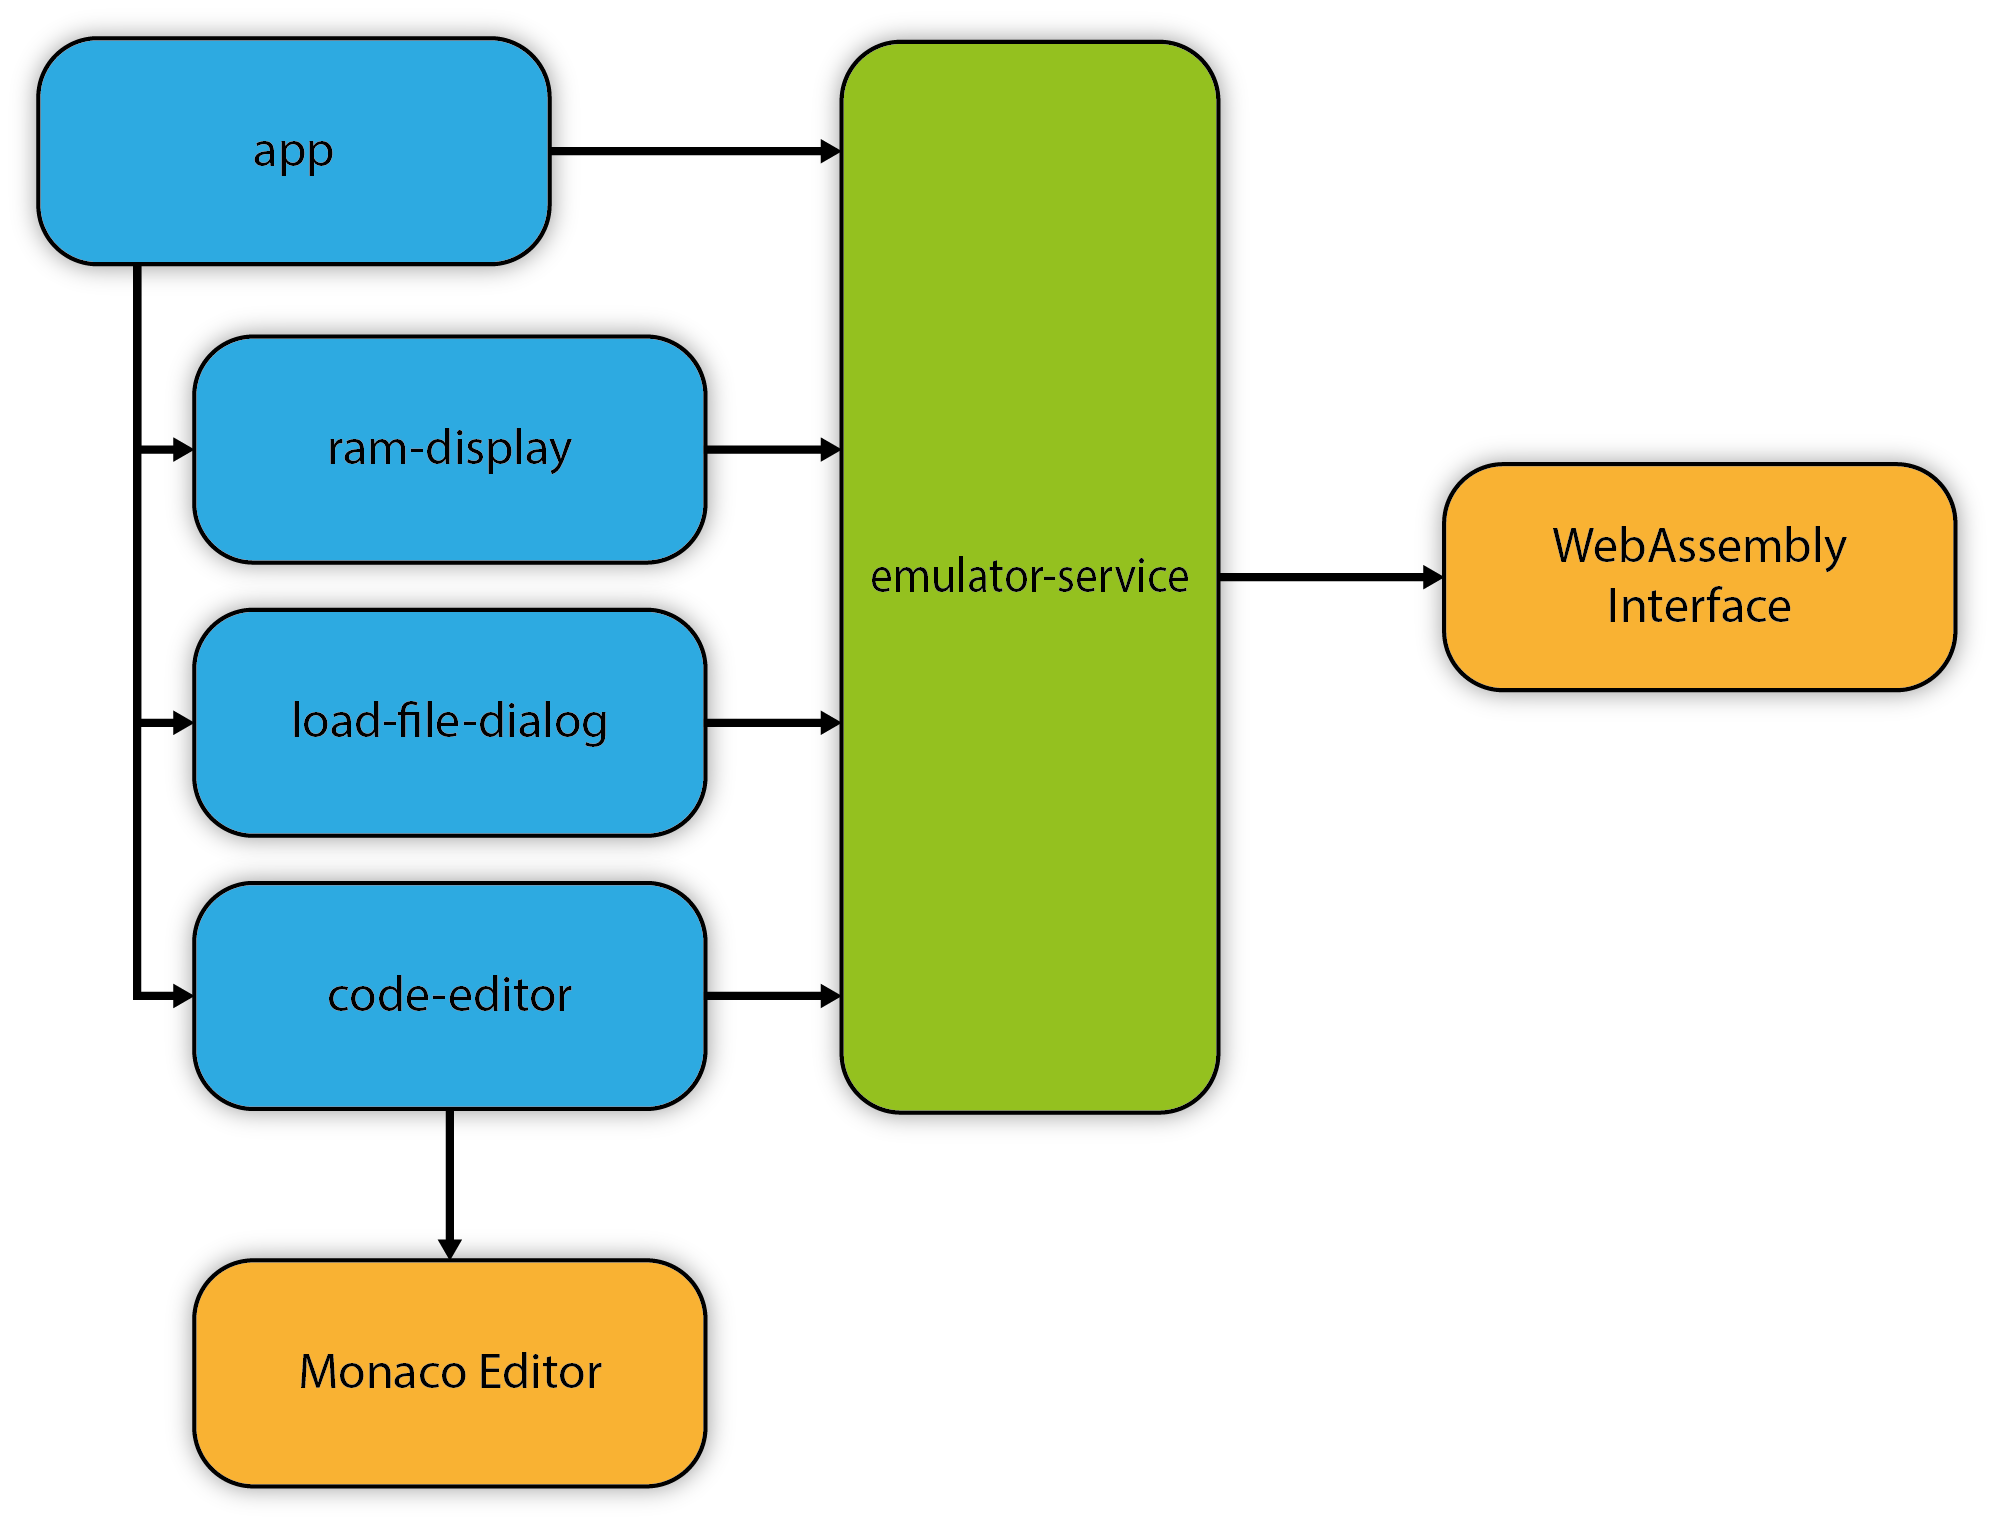
\includegraphics[width=1.0\textwidth]{Bilder/AngularArchitektur.png}
    \label{fig:architecture}
\end{figure}

In Abbildung \ref{fig:architecture} ist die Architektur der Applikation veranschaulicht. Die blauen Objekte stellen Komponenten dar, das grüne Objekt den Service und die orangenen Objekte externe Abhängigkeiten.

\subsection{Komponenten}

\subsubsection{App-Component}

Die App-Component bildet den zentralen Zugangspunkt der meisten Angular-Applikationen. Von hier aus werden die anderen Komponenten der Anwendung eingebunden und miteinander verknüpft.
Das HTML-Template der App-Component umfasst in diesem Fall das komplette Skelett der Anwendung, welches eine Titelleiste und die Einteilung in eine linke und eine rechte Hälfte definiert.
In dieses Skelett werden dann die anderen Komponenten eingebunden.

\subsubsection{\ac{RAM}-Display}

Die \ac{RAM}-Display-Component stellt den Arbeitsspeicher des Emulators in Form einer 16x16 Matrix dar. Genutzt wird dafür eine einfache HTML-Tabelle, die mithilfe von Stylesheets entsprechend angepasst wird. Der Zugriff auf den Arbeitsspeicher erfolgt durch direkten Zugriff auf den Speicherbereich der \ac{WASM}-Objekte im Browser über einen Pointer.

Neben der Arbeitsspeicher-Matrix kümmert sich diese Komponente auch um die Anzeige der verschiedenen Register.

\subsubsection{Load-File-Dialog}

Diese Komponente wird nicht von Anfang an auf der Seite eingebunden, sondern wird erst dann in Form eines modalen Dialogs angezeigt, wenn der Nutzer auf den \textit{Load}-Button in der Aktionsleiste drückt. Der Dialog zeigt dann ein simples HTML-Formular an, das mit einem \mintinline{html}{<input type="file"/>} eine Dateiauswahl ermöglicht.

\subsubsection{Code-Editor}

Die Code-Editor-Component ermöglicht der Anwendung die Nutzung der Monaco Editor Bibliothek. Dazu erfolgt eine umfangreiche Konfiguration des Editors, um beispielsweise die Tokens und das Farbschema für das Syntaxhighlighting festzulegen oder um die Autovervollständigung zu ermöglichen.

\subsection{Emulator-Service}

Alle Komponenten greifen über das Dependency-Injection-Framework von Angular auf den sogenannten Emulator-Service zu. Dieser Service verwaltet den Emulator, der mithilfe des in Kapitel \ref{sec:wasmapi} definierten \ac{WASM}-Interfaces erstellt wird.

Der Service bietet den Komponenten verschiedene Funktionen an, wie zum Beispiel, Quellcode zu assemblen, was vom \textit{Assemble}-Button in der Aktionsleiste genutzt wird. Zur Ausführung von Programmen wird im Service außerdem die Hauptschleife des Emulators implementiert.

\begin{minted}{typescript}
    this._loop = window.setInterval(() => {
      for (let i = 0; i < this._stepsPerInterval; i++) {
        this.cpuStep();
      }
    }, this._interval);
\end{minted}

Statt einer \rust{while}-Schleife kommt hier die Funktion \ts{window.setInterval()} des Browsers zum Einsatz. Diese Funktion führt eine gegebene andere Funktion periodisch immer wieder mit einem bestimmten Intervall auf. Dies ermöglicht der Webanwendung trotz der \enquote{Endlossschleife} responsiv zu bleiben. Da das Intervall nicht beliebig klein sein kann, gibt es außerdem die Möglichkeit, in jedem Schleifendurchlauf mehrere Prozessorschritte durchzuführen. So kann der Emulator trotzdem so schnell laufen wie es nötig ist.

Die \ts{cpuStep()}-Methode arbeitet nun verschiedene Schritte ab: Hauptaufgabe der Methode ist das Ausführen von \ts{emulator.execute_next()}, was dafür sorgt, dass der Emulator die nächste Instruktion ausführt und den Program Counter gegebenenfalls erhöht. Nach dem Ausführen des Emulatorschritts wird der Arbeitsspeicher mit dem vorherigen Zustand verglichen, um festzustellen ob es eine Änderung gab. Dies wird für das Einfärben der entsprechenden Stelle in der \ac{RAM}-Matrix genutzt.

Eine weitere Aufgabe der Methode ist die Emulation von sogenannten \textit{\ac{CPM} Syscalls}.

\subsection{CP/M Emulation}

Um den Emulator zu testen, wurden einige frei verfügbare Programme genutzt. Diese wurden allerdings für das \ac{CPM}-Betriebssystem geschrieben, welches ab 1974 unter anderem für den Intel 8080 entwickelt wurde und auf diversen Rechnern für Endanwender zum Einsatz kam.

Ein wesentliches Feature, was diese Programme nutzen, sind die \ac{BDOS} Syscalls, die auf einem \ac{CPM} System das Ausgeben von Text in einem Terminal ermöglichen \cite{cpmSyscalls}.

\begin{minted}{asm}
    LD DE   ;parameter
    LD C    ;function
    CALL 5  ;syscall routine
\end{minted}

Für den Aufruf eines Syscalls muss die Funktion, die aufgerufen wird, in das Register C geschrieben werden. Mögliche Parameter können im Register DE abgelegt werden. Der Syscall kann nun durch einen Sprung auf Adresse 5 ausgeführt werden.

Relevant für die Programme, die zum Testen genutzt werden, sind lediglich die Syscalls 2 (Zeichen-Ausgabe) und 9 (String-Ausgabe). Die Emulation dieser Syscalls ist vergleichsweise simpel:

\begin{minted}{typescript}
    if (this._cpmMode) {
      // Patch memory for BDOS syscalls
      this._emulatorMemory[5] = 0xC9; // RET
      this._emulator.pc = 0x100;
    }
\end{minted}

Beim Start eines Programms, was im \ac{CPM} Modus ausgeführt wird, wird der Speicher an der Stelle 5 mit einer Return-Instruktion überschrieben. Das sorgt dafür, dass das Programm bei jedem Syscall sofort wieder an die ursprüngliche Stelle zurückspringt. Zusätzlich wird der Program Counter beim Start direkt auf 0x100 gesetzt, da \ac{CPM} davon ausgeht, dass Nutzerprogramme an dieser Stelle beginnen.

Im \ts{cpuStep()} wird nun folgender Code ausgeführt:

\begin{minted}{typescript}
    if (this.emulator.pc == 0x05) {
        // Emulate CP/M BDOS syscalls
        const syscall = registers.c;
        switch(syscall) {
            case 2: {
                // BDOS function 2 (C_WRITE) - Console output
                const char = registers.e;
                console.log(String.fromCharCode(char));
                break;
            }
            case 9: {
                // BDOS function 9 (C_WRITESTR) - Output string
                let address = largeRegisters.d;
                let currentChar = "";
                let fullString = "";
                while (currentChar != "$") {
                    fullString += currentChar;
                    const charCode = emulatorMemory[address++];
                    currentChar = String.fromCharCode(charCode);
                }
                console.log(fullString);
                break;
            }
        }
    }
\end{minted}

Sobald der Program Counter den Wert 5 hat, das Programm also an die Syscall Adresse gesprungen ist, wird der entsprechende Syscall emuliert. Beim Syscall 2 wird das Zeichen, was sich in Register E befindet, ausgegeben. Syscall 9 gibt den String, der sich an der Speicheradresse aus Register DE befindet, so lange aus, bis das Zeichen \enquote{\$} auftritt.